\section{Task Parallelism}

\begin{frame}{Parallelism in \OCamlFive}
\Large
\begin{itemize}
  \setlength\itemsep{2em}
  \item
    Domains
    \begin{itemize}
      \item \ocamlinline{Domain.spawn : (unit -> 'a) -> 'a Domain.t}
      \item \ocamlinline{Domain.join : 'a Domain.t -> 'a}
    \end{itemize}
  \item
    Atomic primitives
    \begin{itemize}
      \item Atomic references (\ocamlinline{'a Atomic.t})
      \item Atomic record fields (\ocamlinline{'a Atomic.Loc.t})
    \end{itemize}
\end{itemize}
\end{frame}

\begin{frame}[fragile]{Fibonacci Using Domains}
\large
\begin{ocamlcode}
let rec fibonacci n =
  if n <= 1 then
    1
  else
    let dom1 = Domain.spawn (fun () -> fibonacci (n - 1)) in
    let dom2 = Domain.spawn (fun () -> fibonacci (n - 2)) in
    Domain.join dom1 + Domain.join dom2
\end{ocamlcode}
\begin{overbox}<2>
  \Large
  \textbf{This implementation is \emph{wrong}:}
  \begin{itemize}
    \item the number of active domains is limited;
    \item performance collapses when spawning more domains than available cores.
  \end{itemize}
\end{overbox}
\end{frame}

\begin{frame}[fragile]{Fibonacci Using a Parallel Scheduler}
\begin{adjustwidth}{-1em}{-1em}
\large
\begin{ocamlcode}
let rec fibonacci ctx n =
  if n <= 1 then
    1
  else
    let fut1 = Future.async ctx (fun ctx -> fibonacci ctx (n - 1)) in
    let fut2 = Future.async ctx (fun ctx -> fibonacci ctx (n - 2)) in
    Future.wait ctx fut1 + Future.wait ctx fut2

let fibonacci num_domain n =
  let pool = Pool.create num_domain in
  let res = Pool.run_on pool (fun ctx -> fibonacci ctx n) in
  Pool.close pool ;
  res
\end{ocamlcode}
\end{adjustwidth}
\end{frame}

\begin{frame}{Existing Parallel Schedulers}
\centering
\Large
\begin{tabular}{c@{\hskip3em}c@{\hskip3em}c@{\hskip3em}c}
      
\includegraphics[height=4em]{images/ocaml.png}
    &
      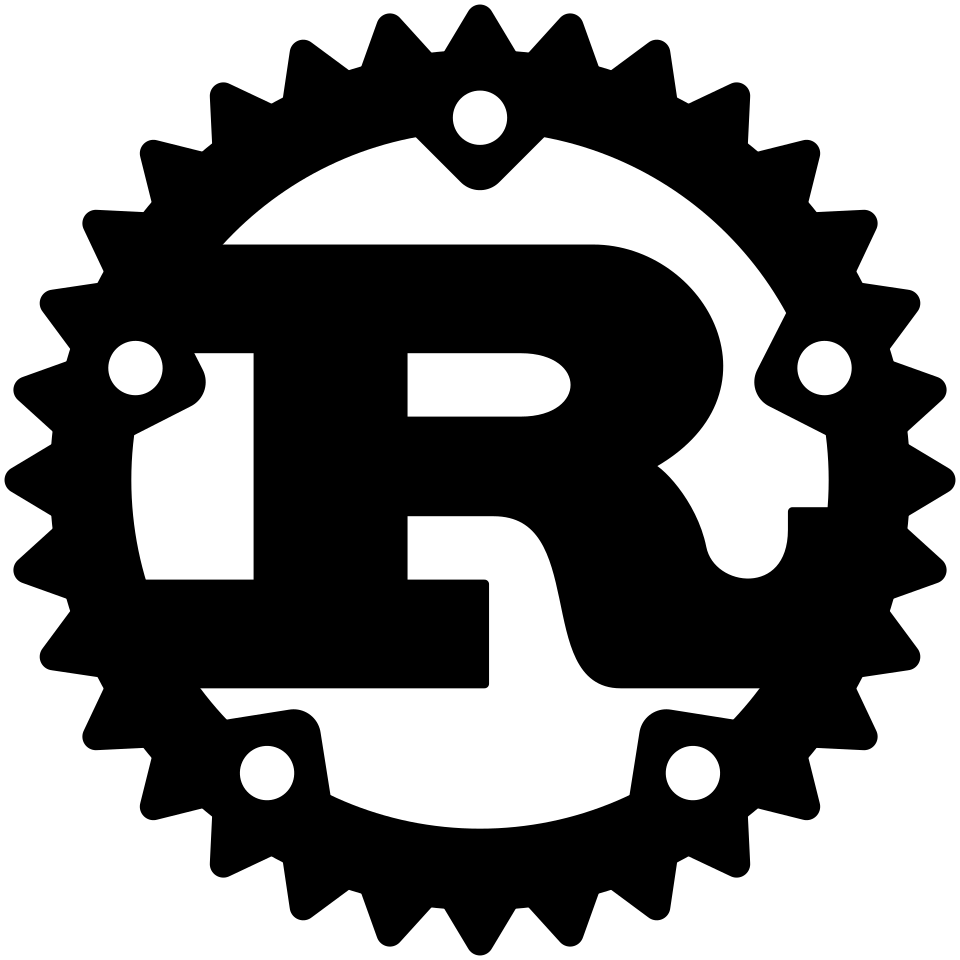
\includegraphics[height=4em]{images/rust.png}
    &
      
\includegraphics[height=4em]{images/cpp.png}
    &
      
\includegraphics[height=4em]{images/go.png}
  \\\\
      \Domainslib
    &
      \Rayon
    &
      \Cilk
    &
      Goroutines
  \\
      \Moonpool
    &
      \Tokio
    &
      \TBB
    &
  \\
    &
    &
      \Taskflow
    &
\end{tabular}
\end{frame}

\begin{frame}{Work-Stealing}
\centering
\input{figures/work_stealing}
\end{frame}
